\documentclass[a4paper,12pt,oneside]{book}%extreport
\usepackage{times} 
% \usepackage{multibib}
\usepackage{lipsum}
\usepackage{appendix}
\usepackage[shortlabels]{enumitem}
\usepackage{booktabs}
\usepackage{rotating} % Rotating table
\usepackage{hhline}
\usepackage{colortbl}
\usepackage{afterpage}
\usepackage{mathtools} %Fixes/improves amsmath
\usepackage{setspace}
\usepackage[utf8]{vietnam} 
\usepackage{amstext, amsmath,latexsym,amsbsy,amssymb, amssymb,amsthm,amsfonts,multicol, nccmath}
\usepackage[left=3cm,right=2cm,top=2.0cm,bottom=2cm,footskip=40pt]{geometry}
\usepackage{pdflscape}
\usepackage{apacite}
\usepackage{tikz}
\usepackage{array}
\newcolumntype{C}[1]{>{\centering\let\newline\\\arraybackslash\hspace{0pt}}m{#1}}
\usetikzlibrary{calc}
\usepackage{tabularx}
\usepackage{multicol}
\usepackage{array,color,colortbl}
\setcounter{secnumdepth}{4}
%\usepackage[square,numbers]{natbib}
\usepackage[square, comma, numbers, sort&compress]{natbib}
\setlength{\parindent}{1cm}
\usepackage{color}
\usepackage{indentfirst}
\usepackage{exscale,eucal}
\usepackage{fancyhdr}
\usepackage{fncychap}
\usepackage[chapter]{algorithm}
\usepackage{multirow}
\usepackage{graphicx}
\usepackage{algpseudocode}
\usepackage{tabularx,multicol,multirow,longtable}
\usepackage{etoolbox}
\usepackage{tikz}	\usetikzlibrary{calc,arrows,decorations.pathmorphing,backgrounds,positioning,fit,shapes,decorations.shapes, shapes.geometric, decorations.pathreplacing, decorations.text}

\tikzstyle{block} = [draw,rectangle,thick,minimum height=2em,minimum width=2em,drop shadow,fill=blue!50]
\tikzstyle{sum} = [draw,circle,inner sep=0mm,minimum size=2mm]
\tikzstyle{connector} = [->,thick]
\tikzstyle{line} = [very thick]
\tikzstyle{branch} = [circle,inner sep=0pt,minimum size=1mm,fill=black,draw=black]
\tikzstyle{axes} = [->,>=stealth',semithick]
\tikzstyle{important line} = [very thick,draw=red]
\tikzstyle{important text} = [rounded corners,fill=red!10,inner sep=1ex]
\usepackage{circuitikz}
\usepackage{pgfplots}
\usepackage[numbers]{natbib}
\usepackage{titlesec}
\usepackage[labelsep=period]{caption}
\usepackage{subfigure}
\DeclareCaptionFormat{myformat}{\fontsize{13}{15}\selectfont#1#2#3}
\captionsetup{format=myformat}
\usepackage{titletoc}
\titlelabel{\thetitle.\,\,}
\titleformat{\chapter}[display] 
{\fontsize{14}{16}\selectfont\bfseries\centering}
{\MakeUppercase{\chaptertitlename}\ \thechapter}{0pt}{\fontsize{14}{16}\selectfont\MakeUppercase}
\titlespacing{\chapter}{0pt}{0pt}{40pt} 
\titleformat*{\section}{\fontsize{14}{14}\selectfont\bfseries}
\titleformat*{\subsection}{\fontsize{14}{14}\selectfont\bfseries\slshape}
\titleformat*{\subsubsection}{\fontsize{14}{14}\slshape}
\titleformat*{\paragraph}{\large\bfseries}
\titleformat*{\subparagraph}{\large\bfseries}
\graphicspath {{figures/}}

\titlespacing\section{0pt}{6pt plus 4pt minus 2pt}{1pt plus 2pt minus 2pt} 
\titlespacing\subsection{0pt}{6pt plus 4pt minus 2pt}{1pt plus 2pt minus 2pt}
\titlespacing\subsubsection{0pt}{6pt plus 4pt minus 2pt}{0pt plus 2pt minus 2pt}
\titlespacing\subsubsubsection{0pt}{6pt plus 4pt minus 2pt}{0pt plus 2pt minus 2pt}

\usepackage[subfigure]{tocloft} 

\cftsetpnumwidth{20pt}
\titlecontents{chapter}
[0pt]
{}
{\fontsize{13.5}{14}\selectfont\MakeUppercase{\chaptername}\ \thecontentslabel.\,\,}
{}
{\cftdotfill{\cftdotsep}\contentspage} 
\renewcommand{\cftsecaftersnum}{.}%
\renewcommand{\cftsubsecaftersnum}{.}%

\usetikzlibrary{calc}
\newtheorem{definition}{\bf Định nghĩa}[chapter]
\newtheorem{theorem}{\bf Định lý}[chapter]
\newtheorem{lemma}{\bf Bổ đề}[chapter]

\renewcommand{\cftfigfont}{Hình~}
\renewcommand{\cfttabfont}{Bảng~ }
\floatname{algorithm}{Thuật toán}
\makeatletter
\renewcommand\@biblabel[1]{[#1]}
\renewcommand\harvardyearleft{\unskip~(}
\renewcommand\harvardyearright{\unskip )}
\makeatother
\renewcommand{\baselinestretch}{1.4}
\flushbottom
\renewcommand*{\bibfont}{\fontsize{13}{16}\selectfont}

\usepackage[hidelinks, unicode]{hyperref}

\begin{document}
	%%% List of new cmds:


% Line
\tikzset{
    line/.style={draw, thick},
}

% Node S
\newcommand{\NodeS}[5]{\NodeSS{3mm}{draw=black, line width=1pt, fill=teal!30!white}{#4}{#5};
\node (#1) at (#2, #3) [node S, draw=black, fill=teal!10!white] {}
}
\newcommand{\NodeSS}[4]{
    \tikzset{
        old inner xsep/.estore in=\oldinnerxsep,
        old inner ysep/.estore in=\oldinnerysep,
        node S/.style 2 args={
            circle,
            old inner xsep=\pgfkeysvalueof{/pgf/inner xsep},
            old inner ysep=\pgfkeysvalueof{/pgf/inner ysep},
            /pgf/inner xsep=\oldinnerxsep+#1,
            /pgf/inner ysep=\oldinnerysep+#1,
            alias=sourcenode,
            append after command={
            let     \p1 = (sourcenode.center),
                    \p2 = (sourcenode.east),
                    \n1 = {\x2-\x1-#1-0.5*\pgflinewidth}
            in
                node [inner sep=#3, draw, fill, circle, minimum width=2*\n1,at=(\p1), #2] {#4}     % Outside box
            }
        },
        node S/.default={3mm}{black}     % inside  
    }
}

% Node R
\newcommand{\NodeR}[5]{\NodeRR{3mm}{draw=black, line width=1pt, fill=green!30!white}{#4}{#5};
\node (#1) at (#2, #3) [node R, draw=black, fill=green!10!white] {}
}
\newcommand{\NodeRR}[4]{
    \tikzset{
        old inner xsep/.estore in=\oldinnerxsep,
        old inner ysep/.estore in=\oldinnerysep,
        node R/.style 2 args={
            circle,
            old inner xsep=\pgfkeysvalueof{/pgf/inner xsep},
            old inner ysep=\pgfkeysvalueof{/pgf/inner ysep},
            /pgf/inner xsep=\oldinnerxsep+#1,
            /pgf/inner ysep=\oldinnerysep+#1,
            alias=sourcenode,
            append after command={
            let     \p1 = (sourcenode.center),
                    \p2 = (sourcenode.east),
                    \n1 = {\x2-\x1-#1-0.5*\pgflinewidth}
            in
                node [inner sep=#3, draw, fill, circle, minimum width=2*\n1,at=(\p1), #2] {#4}     % Outside box
            }
        },
        node R/.default={3mm}{black}     % inside  
    }
}

% Node E
\newcommand{\NodeE}[5]{\NodeEE{3mm}{draw=black, line width=1pt, fill=red!30!white}{#4}{#5};
\node (#1) at (#2, #3) [node E, draw=black, fill=red!10!white] {}
}
\newcommand{\NodeEE}[4]{
    \tikzset{
        old inner xsep/.estore in=\oldinnerxsep,
        old inner ysep/.estore in=\oldinnerysep,
        node E/.style 2 args={
            circle,
            old inner xsep=\pgfkeysvalueof{/pgf/inner xsep},
            old inner ysep=\pgfkeysvalueof{/pgf/inner ysep},
            /pgf/inner xsep=\oldinnerxsep+#1,
            /pgf/inner ysep=\oldinnerysep+#1,
            alias=sourcenode,
            append after command={
            let     \p1 = (sourcenode.center),
                    \p2 = (sourcenode.east),
                    \n1 = {\x2-\x1-#1-0.5*\pgflinewidth}
            in
                node [inner sep=#3, draw, fill, circle, minimum width=2*\n1,at=(\p1), #2] {#4}     % Outside box
            }
        },
        node E/.default={3mm}{black, line width=1pt, fill=red!30!white}     % inside  
    }
}

% Node D
\newcommand{\NodeD}[5]{\NodeDD{3mm}{draw=black, line width=1pt, fill=blue!30!white}{#4}{#5};
\node (#1) at (#2, #3) [node D, draw=black, fill=blue!10!white] {}
}
\newcommand{\NodeDD}[4]{
    \tikzset{
        old inner xsep/.estore in=\oldinnerxsep,
        old inner ysep/.estore in=\oldinnerysep,
        node D/.style 2 args={
            circle,
            old inner xsep=\pgfkeysvalueof{/pgf/inner xsep},
            old inner ysep=\pgfkeysvalueof{/pgf/inner ysep},
            /pgf/inner xsep=\oldinnerxsep+#1,
            /pgf/inner ysep=\oldinnerysep+#1,
            alias=sourcenode,
            append after command={
            let     \p1 = (sourcenode.center),
                    \p2 = (sourcenode.east),
                    \n1 = {\x2-\x1-#1-0.5*\pgflinewidth}
            in
                node [inner sep=#3, draw, fill, circle, minimum width=2*\n1,at=(\p1), #2] {#4}     % Outside box
            }
        },
        node D/.default={3mm}{black, line width=1pt, fill=blue!30!white}     % inside 
    }
}

% XOR symbol
\tikzset{XOR/.style={draw,circle,append after command={
        [shorten >=\pgflinewidth, shorten <=\pgflinewidth,]
        (\tikzlastnode.north) edge (\tikzlastnode.south)
        (\tikzlastnode.east) edge (\tikzlastnode.west)
        }
    }
}


% circle dot line
\tikzset{decorate sep/.style 2 args=
{decorate,decoration={shape backgrounds,shape=circle,shape size=#1,shape sep=#2}}}

% NNN
\newcommand{\NNN}{
    \newcommand{\inputnum}{4} 
    \newcommand{\numhiddenlayer}{2}
    \newcommand{\hiddennum}{5}  
    \newcommand{\outputnum}{1} 
    
    \begin{tikzpicture}
        % Input Layer
        \foreach \i in {1,...,\inputnum}
        {
            \node[circle, 
                minimum size = 6mm,
                fill=orange!30] (Input-\i) at (0,-\i) {};
        }
        \foreach \i in {1,...,3}
        {
            \draw node [circle, fill=orange!30, scale=0.5] at (0, -\i - 0.5) {};
        }
         
        % Hidden Layer
        \foreach \i in {1,...,\numhiddenlayer}
        {
        \foreach \j in {1,...,\hiddennum}
            {
                \node[circle, 
                    minimum size = 6mm,
                    fill=teal!50,
                    yshift=(\hiddennum-\inputnum)*5 mm
                ] (Hidden-\i-\j) at (2.5 * \i,-\j) {};
            }
        \foreach \j in {1,...,4}
            {
                \draw node [circle, fill=teal!50, scale=0.5] at (2.5 * \i, -\j) {};
            }    
        }
        
        % Output Layer
        \foreach \i in {1,...,\outputnum}
        {
            \node[circle, 
                minimum size = 6mm,
                fill=purple!50,
                yshift=(\outputnum-\inputnum)*5 mm
            ] (Output-\i) at (7,-\i) {};
        }
         
        % Connect neurons In-Hidden
        \foreach \i in {1,...,\inputnum}
        {
            \foreach \j in {1,...,\hiddennum}
            {
                \draw[->, shorten >=1pt, -stealth] (Input-\i) -- (Hidden-1-\j);   
            }
        }
         
        % Connect neurons Hidden-Hidden
        \foreach \i in {1,...,\hiddennum}
        {
            \foreach \j in {1,...,\hiddennum}
            {
                \draw[->, shorten >=1pt, -stealth] (Hidden-1-\i) -- (Hidden-2-\j);   
            }
        }
         
        % Connect neurons Hidden-Out
        \foreach \i in {1,...,\hiddennum}
        {
            \foreach \j in {1,...,\outputnum}
            {
                \draw[->, shorten >=1pt, -stealth] (Hidden-\numhiddenlayer-\i) -- (Output-\j);
            }
        }
        
        % Inputs
        \foreach \i in {2,...,2}
        {            
            \draw[<-, line width = 2pt, stealth-] ([xshift=-10pt]Input-\i.west) -- ++(-1,0)
                node[left, label=$X_n$]{};
        }
        \foreach \i in {3,...,3}
        {            
            \draw[<-, line width = 2pt, stealth-] ([xshift=-10pt]Input-\i.west) -- ++(-1,0)
                node[left, label=$Y_n / Z_n$]{};
        }
         
        % Outputs
        \foreach \i in {1,...,\outputnum}
        {            
            \draw[<-, line width = 2pt, -stealth] (Output-\i) -- ++(2,0)
                node[pos=0.3,right, label={$T(x_k, y_k / z_k)$}]{};
        }
    \end{tikzpicture}
}

\tikzstyle{startstop} = [rectangle, rounded corners, minimum width=3cm, minimum height=1cm,text centered, draw=black, fill=red!10!white]

\tikzstyle{io} = [trapezium, trapezium left angle=70, trapezium right angle=110, minimum width=3cm, minimum height=1cm, text centered, draw=black, fill=orange!10!white]

\tikzstyle{process} = [rectangle, minimum width=3cm, minimum height=1cm, text centered, draw=black, fill=blue!10!white]

\tikzstyle{decision} = [diamond, minimum width=3cm, minimum height=1cm, text centered, draw=black, fill=green!10!white]

\tikzstyle{arrow} = [thick,->,>=stealth]

\tikzstyle{darrow} = [thick, stealth-stealth]

\tikzstyle{arrowt1}  = [thick,->,>=stealth, draw=red]

\tikzstyle{arrowt2}  = [thick,->,>=stealth, dashed, draw=green]

\tikzstyle{arrowt3}  = [thick,->,>=stealth, dotted, draw=black]

\tikzstyle{field} = [rectangle, minimum width=5mm, minimum height=10mm, align=center, fill=green!10!white, font=\footnotesize, draw=black, line width=1pt]

\tikzstyle{field1} = [rectangle, minimum width=20mm, minimum height=5mm, align=center, fill=green!10!white, font=\scriptsize, draw=black, line width=1pt, rotate=-90]

\tikzstyle{field2} = [rectangle, minimum width=5mm, minimum height=20mm, align=center, fill=green!10!white, font=\scriptsize, draw=black, line width=1pt]

\tikzstyle{field3} = [rectangle, minimum width=31mm, minimum height=5mm, align=center, fill=green!10!white, font=\small, draw=black, line width=1pt, rotate=-90]

\tikzstyle{field4} = [rectangle, minimum width=31mm, minimum height=5mm, align=center, fill=green!10!white, draw=black, line width=1pt, rotate=-90]

\tikzstyle{field5} = [rectangle, minimum width=3mm, minimum height=10mm, align=center, fill=green!10!white, draw=black, line width=1pt]

\tikzstyle{field6} = [rectangle, minimum width=15mm, minimum height=10mm, align=center, fill=green!10!white, draw=black, line width=1pt]

\tikzstyle{field7} = [rectangle, minimum width=3mm, minimum height=10mm, align=center, fill=green!10!white, font=\footnotesize, draw=black, line width=1pt]

\tikzstyle{field8} = [rounded rectangle, minimum width=10mm, minimum height=10mm, align=center, fill=green!10!white, draw=black, line width=1pt]

\makeatletter
\tikzset{
    database/.style={
        path picture={
            \draw (0, 1.5*\database@segmentheight) circle [x radius=\database@radius,y radius=\database@aspectratio*\database@radius];
            \draw (-\database@radius, 0.5*\database@segmentheight) arc [start angle=180,end angle=360,x radius=\database@radius, y radius=\database@aspectratio*\database@radius];
            \draw (-\database@radius,-0.5*\database@segmentheight) arc [start angle=180,end angle=360,x radius=\database@radius, y radius=\database@aspectratio*\database@radius];
            \draw (-\database@radius,1.5*\database@segmentheight) -- ++(0,-3*\database@segmentheight) arc [start angle=180,end angle=360,x radius=\database@radius, y radius=\database@aspectratio*\database@radius] -- ++(0,3*\database@segmentheight);
        },
        minimum width=2*\database@radius + \pgflinewidth,
        minimum height=3*\database@segmentheight + 2*\database@aspectratio*\database@radius + \pgflinewidth,
    },
    database segment height/.store in=\database@segmentheight,
    database radius/.store in=\database@radius,
    database aspect ratio/.store in=\database@aspectratio,
    database segment height=0.1cm,
    database radius=0.25cm,
    database aspect ratio=0.35,
}
\makeatother
	
	\pagestyle{empty}
	\begin{titlepage}
\centering
\begin{tikzpicture}[overlay,remember picture]
    \centering
    \draw[line width = 3pt] ($(current page.north west) + (1.115in,-0.5in)$) rectangle ($(current page.south east) + (-0.6in,0.6in)$);
    \draw (0,-25.5) node[above]{\fontsize{12}{12}\selectfont{\textbf{Hà Nội - 2023}}};
\end{tikzpicture}
\vspace{-1.5cm}
\begin{center}
\MakeUppercase{{\fontsize{12}{12}\selectfont{ĐẠI HỌC QUỐC GIA HÀ NỘI}}}

\noindent{\textbf {\MakeUppercase{\fontsize{12}{12}\selectfont {TRƯỜNG ĐẠI HỌC CÔNG NGHỆ}}}}\\
%}
	\vspace{-0.5cm}
%\noindent\rule{10cm}{0.7pt}
\vspace{2cm}
\begin{figure} [!htb]
	\centering
	
\includegraphics[width=0.2\linewidth]{figures/UET.png}
	\label{fig:uetlogo}
\end{figure}
\vspace{1.5cm}

		
	{\textbf {\fontsize{14}{14}\selectfont{ĐỖ HẢI SƠN}}}\\
	\vspace{2cm}
{
{\textbf {\MakeUppercase{\fontsize{17}{17}\selectfont{NGHIÊN CỨU NHẬN DẠNG HỆ THỐNG}}}}\\[3pt]
{\textbf {\MakeUppercase{\fontsize{17}{17}\selectfont{VỚI TRI THỨC MỚI CHO HỆ THỐNG TRUYỀN THÔNG}}}}\\[3pt]
{\textbf {\MakeUppercase{\fontsize{17}{17}\selectfont{MIMO KÍCH THƯỚC LỚN}}}}\\[3pt]
}
\vspace{3cm}
\MakeUppercase{\textbf{\fontsize{14}{14}\selectfont{{LUẬN VĂN THẠC SĨ}}}}\\[3pt]
\MakeUppercase{\textbf{\fontsize{14}{14}\selectfont{{NGÀNH CÔNG NGHỆ KỸ THUẬT ĐIỆN TỬ, TRUYỀN THÔNG}}}}\\[3pt]
\end{center}


\end{titlepage}
	\newpage
	\pagestyle{plain}
	\pagenumbering{gobble}
	\begin{center}
    \begin{tikzpicture}[overlay,remember picture]
        \centering
        \draw[line width = 3pt] ($(current page.north west) + (1.115in,-0.5in)$) rectangle ($(current page.south east) + (-0.6in,0.6in)$);
        \draw (0,-25.5) node[above]{\fontsize{12}{12}\selectfont{\textbf{Hà Nội - 2023}}};
    \end{tikzpicture}
\end{center}
\vspace{-1.5cm}

\begin{center}
    {\MakeUppercase{\fontsize{12}{12}\selectfont{ĐẠI HỌC QUỐC GIA HÀ NỘI}}}
    
    \noindent\textbf {\MakeUppercase{\fontsize{12}{12}\selectfont{TRƯỜNG ĐẠI HỌC CÔNG NGHỆ}}}\\

    \vspace{1.5cm}
    
    {\textbf {\fontsize{14}{14}\selectfont{ĐỖ HẢI SƠN}}}\\
    \vspace{1.5cm}
    
    {\textbf {\MakeUppercase{\fontsize{17}{17}\selectfont{NGHIÊN CỨU NHẬN DẠNG HỆ THỐNG}}}}\\[3pt]
    {\textbf {\MakeUppercase{\fontsize{17}{17}\selectfont{VỚI TRI THỨC MỚI CHO HỆ THỐNG TRUYỀN THÔNG}}}}\\[3pt]
    {\textbf {\MakeUppercase{\fontsize{17}{17}\selectfont{MIMO KÍCH THƯỚC LỚN}}}}\\[3pt]
\end{center}
\vspace{1.5cm}

Ngành: Công nghệ kỹ thuật điện tử, truyền thông\\
\indent Chuyên ngành: Kỹ thuật viễn thông\\ 
\indent Mã số: 8510302.02\\

\vspace{1.5cm}
\begin{center}
    \MakeUppercase{\textbf{\fontsize{14}{14}\selectfont{{LUẬN VĂN THẠC SĨ}}}}\\[3pt]
    \MakeUppercase{\textbf{\fontsize{14}{14}\selectfont{{NGÀNH CÔNG NGHỆ KỸ THUẬT ĐIỆN TỬ, TRUYỀN THÔNG}}}}\\[3pt]
\end{center}
\vspace{1.5cm}
\begin{tabularx}
    {\linewidth}{>{\setlength\hsize{.0\hsize}}X>{\setlength\hsize{0.9\hsize}}X}
                            & \fontsize{14}{14}\textbf{\selectfont{NGƯỜI HƯỚNG DẪN KHOA HỌC: TS. Trần Thị Thúy Quỳnh}}
\end{tabularx}
	\newpage
	\begin{center}
    \begin{tikzpicture}[overlay,remember picture]
        \centering
        \draw[line width = 3pt] ($(current page.north west) + (1.115in,-0.5in)$) rectangle ($(current page.south east) + (-0.6in,0.6in)$);
        \draw (0,-25.5) node[above]{\fontsize{12}{12}\selectfont{\textbf{Hà Nội - 2023}}};
    \end{tikzpicture}
\end{center}
\vspace{-1.5cm}

\begin{center}
    {\MakeUppercase{\fontsize{12}{12}\selectfont{ĐẠI HỌC QUỐC GIA HÀ NỘI}}}
    
    \noindent\textbf {\MakeUppercase{\fontsize{12}{12}\selectfont{TRƯỜNG ĐẠI HỌC CÔNG NGHỆ}}}\\

    \vspace{1.5cm}
    
    {\textbf {\fontsize{14}{14}\selectfont{ĐỖ HẢI SƠN}}}\\
    \vspace{1.5cm}
    
    {\textbf {\MakeUppercase{\fontsize{17}{17}\selectfont{NGHIÊN CỨU NHẬN DẠNG HỆ THỐNG}}}}\\[3pt]
    {\textbf {\MakeUppercase{\fontsize{17}{17}\selectfont{VỚI TRI THỨC MỚI CHO HỆ THỐNG TRUYỀN THÔNG}}}}\\[3pt]
    {\textbf {\MakeUppercase{\fontsize{17}{17}\selectfont{MIMO KÍCH THƯỚC LỚN}}}}\\[3pt]
\end{center}
\vspace{1.5cm}

Ngành: Công nghệ kỹ thuật điện tử, truyền thông\\
\indent Chuyên ngành: Kỹ thuật viễn thông\\ 
\indent Mã số: 8510302.02\\

\vspace{1.5cm}
\begin{center}
    \MakeUppercase{\textbf{\fontsize{14}{14}\selectfont{{TÓM TẮT LUẬN VĂN THẠC SĨ}}}}\\[3pt]
    \MakeUppercase{\textbf{\fontsize{14}{14}\selectfont{{NGÀNH CÔNG NGHỆ KỸ THUẬT ĐIỆN TỬ, TRUYỀN THÔNG}}}}\\[3pt]
\end{center}
	\newpage
	\def\baselinestretch{1.3}
	\pagestyle{plain}
	\pagenumbering{gobble}
	\clearpage
\phantomsection

\addcontentsline{toc}{chapter}{Lời cam đoan}
\chapter*{Lời cam đoan}

Tôi xin cam đoan luận văn thạc sĩ \textbf{Nghiên cứu nhận dạng hệ thống với tri thức mới cho hệ thống truyền thông MIMO kích thước lớn} là công trình nghiên cứu thực sự của tôi, được thực hiện dựa trên cơ sở lý thuyết, kiến thức chuyên ngành dưới sự hướng dẫn khoa học của TS.~Trần Thị Thúy Quỳnh.

Tôi xin cam đoan những công việc trong luận văn thực hiện chưa từng được các tác giả khác đề xuất. Với sự hiểu biết của mình, tôi chắc chắn các số liệu, kết quả trong luận văn là trung thực và chưa được công bố ở đâu và trong bất cứ công trình nào trừ công trình của tác giả và tài liệu tham khảo.

Nếu có gì sai trái, tôi xin hoàn toàn chịu trách nhiệm.

\vspace{1cm}
\hspace{7cm}\textit{Hà Nội, ngày ... tháng ... năm 2023}

\hspace{9.4cm}\textbf{Học viên}
\vspace{2.5cm}


\hspace{9.3cm}\textbf{Đỗ Hải Sơn}
	\newpage
	\clearpage
\phantomsection

\addcontentsline{toc}{chapter}{Lời cảm ơn}
\chapter*{Lời cảm ơn}

\textit{Tôi xin chân thành cảm ơn TS. Trần Thị Thúy Quỳnh, người đã dẫn dắt, định hướng cho nghiên cứu nhận dạng hệ thống với tri thức mới cho hệ thống truyền thông MIMO kích thước lớn. Tôi cũng xin cảm ơn các thầy, cô Khoa Điện tử - Viễn thông, các thành viên của Viện Tiên tiến về Kỹ thuật và Công nghệ, cùng các thầy, cô phản biện đã cho nhiều góp ý quan trọng, giúp tôi khắc phục những điểm còn hạn chế trong luận văn.}

\textit{Nghiên cứu này được tài trợ bởi Quỹ Phát triển khoa học và công nghệ Quốc gia (NAFOSTED) trong đề tài mã số: 01/2019/TN.}

\textit{Xin gửi lời cảm ơn đến Giáo sư Karim Abed-Meraim và các thành viên thuộc phòng thí nghiệm PRISME, Đại học Orleans, Cộng hoà Pháp đã tận tình giúp đỡ, hướng dẫn tôi trong quá trình tôi là thực tập sinh tại phòng thí nghiệm PRISME từ tháng 09/2022 đến 12/2022.}

\textit{Cuối cùng, tôi xin được gửi lời cảm ơn đến già đình, bạn bè đã luôn bên cạnh động viên, khích lệ, và giúp đỡ tôi trong suốt thời gian qua.}

\textit{Trong quá trình thực hiện luận văn, do thời gian, kiến thức, và điều kiện nghiên cứu còn một số hạn chế nên không tránh khỏi thiếu sót, rất mong nhận được ý kiến đóng góp từ người đọc để tôi có thể tiếp tục phát triển hướng nghiên cứu này.} 

\vspace{1cm}
\hspace{7cm}\textit{Hà Nội, ngày ... tháng ... năm 2023}

\hspace{9.4cm}\textbf{Học viên}
\vspace{2.5cm}


\hspace{9.3cm}\textbf{Đỗ Hải Sơn} 
	\newpage
	\clearpage
\phantomsection

\addcontentsline{toc}{chapter}{Tóm tắt}
\chapter*{\fontsize{13}{13}\selectfont{Tóm tắt}}
\fontsize{12}{12}\selectfont{
\noindent\textbf{Tóm tắt:}


\vspace{0.5cm}
\noindent\textit{\textbf{Từ khóa:}} \textit{}
}
	\newpage
	\pagenumbering{roman}
	
	
	\setlength{\parindent}{1cm}
	\setlength{\parskip}{0.6ex}
	
	\fontsize{13}{16}\selectfont
	\renewcommand{\contentsname}{\vspace{-70pt}\centerline{\fontsize{14}{16}\selectfont\MakeUppercase{Mục lục}}}
	\clearpage
	\phantomsection
	\addcontentsline{toc}{chapter}{Mục lục}
	\tableofcontents
	\clearpage
	\clearpage
\phantomsection

\addcontentsline{toc}{chapter}{Danh mục ký hiệu và chữ viết tắt}
\chapter*{Danh mục ký hiệu và chữ viết tắt}
{\renewcommand{\arraystretch}{1.4}
{\fontsize{12}{13}\selectfont
\begin{longtable}{|C{0.8cm}|>{\raggedright}p{5.4cm}|p{8cm}|}
\hline
\multicolumn{3}{|l|}{\textbf{Danh mục ký hiệu}}\\
\hline
\hline
\textbf{STT} & \textbf{Ký hiệu} & ~\hfill\textbf{Giải thích}\hfill~\\
\hline
1&in thường&Vô hướng\\
\hline
2&in thường, đậm&Vector\\
\hline
3&in hoa, đậm&Ma trận \\
\hline
\end{longtable}
}}
\newpage

{\renewcommand{\arraystretch}{1.2}
{\fontsize{12}{13}\selectfont
\begin{longtable}{|C{0.8cm}|p{1.7cm}|>{\raggedright}p{5.5cm}|p{5.75cm}|}
\hline
\multicolumn{4}{|l|}{\textbf{Danh mục chữ viết tắt}}\\
\hline
\hline
%\multirow{2}{*}{\textbf{STT}} & \textbf{Chữ viết tắt} & ~\hfill\textbf{Giải thích tiếng Anh}\hfill~&~\hfill\textbf{Giải thích tiếng Việt}\hfill~\\
\multirow{2}{*}{\textbf{STT}} & ~\hfill\textbf{Chữ}\hfill~ &\multicolumn{1}{c|}{\multirow{2}{*}{\textbf{Giải thích tiếng Anh}}}&\multicolumn{1}{c|}{\multirow{2}{*}{\textbf{Giải thích tiếng Việt}}}\\
& ~\hfill\textbf{viết tắt}\hfill~ & & \\

\hline
1 & AI & Artificial intelligence & Trí tuệ nhân tạo \\ \hline
2 & AWGN & Additive white Gaussian noise & Tạp âm trắng cộng sinh \\ \hline
3 & B & Blind & Kỹ thuật nhận dạng mù \\ \hline
4 & BER & Bit error rate & Tỷ lệ lỗi bít \\ \hline
5 & CMA & Constant modulus algorithm & Thuật toán mô-đun không đổi \\ \hline
6 & CSI & Channel state information & Thông tin về trạng thái kênh truyền \\ \hline
7 & Data-driven & Data-driven & Hướng dữ liệu \\ \hline
8 & DDCE & Decision-directed channel estimation & Phương pháp hướng quyết định \\ \hline
9 & DetNet & Detection Network & Mạng nơ-ron học sâu phát hiện \\ \hline
10 & DL & Deep learning & Học sâu \\ \hline
11 & DNN & Deep-neural network & Mạng nơ-ron sâu \\ \hline
12 & DoA & Direction of arrival & Hướng sóng đến \\ \hline
13 & DoD & Direction of departure & Hướng phát sóng \\ \hline
14 & FIR & Finite impulse response & Đáp ứng xung hữu hạn \\ \hline
15 & GPR & Gaussian process regression & Thuật toán hồi quy Gaussian \\ \hline
16 & HOS & Higer-order statistics & Đặc tính thống kê bậc cao \\ \hline
17 & I.i.d & Independent and identically distributed & Biến độc lập và phân phối đồng nhất \\ \hline
18 & ICA & Independent component analysis & Phân tích thành phần độc lập \\ \hline
19 & ISD & Iterative sequential detection & Mạng học sâu phát hiện tuần tự lặp lại \\ \hline
20 & LMMSE & Linear Minimum mean square error & Kỹ thuật ước lượng lỗi bình phương trung bình nhỏ nhất tuyến tính \\ \hline
21 & LMS & Least mean squares & Kỹ thuật trung bình bình phương nhỏ nhất \\ \hline
22 & LS & Least square & Kỹ thuật bình phương nhỏ nhất \\ \hline
23 & LSTM & Long/short-term memory & Mạng trí nhớ dài hạn/ngắn hạn \\ \hline
24 & MIMO & Multi-input multi-output & Hệ thống đa đầu vào đa đầu ra \\ \hline
25 & ML & Machine learning & Học máy \\ \hline
26 & MLE & Maximum likelihood estimator & Bộ ước lượng hợp lẽ cực đại \\ \hline
27 & mMIMO & Massive Multi-input multi-output & Hệ thống đa đầu vào đa đầu ra kích thước lớn \\ \hline
28 & MMSE & Minimum mean square error & Kỹ thuật lỗi trung bình phương sai tối thiểu \\ \hline
29 & mmWave & Millimeter wave & Bước sóng mi-li-mét \\ \hline
30 & Model-driven & Model-driven & Hướng mô hình \\ \hline
31 & MRE & Mutually referenced equalizers & Bộ cân bằng kênh tham chiếu \\ \hline
32 & NB & Non-blind & Kỹ thuật nhận dạng không mù \\ \hline
33 & NN & Neural network & Mạng nơ-ron \\ \hline
34 & PC & Pilot contamination & Ô nhiễm pilot \\ \hline
35 & PCA & Principal components analysis & Phân tích thành phần chính \\ \hline
36 & Pilot & Pilot & Ký hiệu hoa tiêu \\ \hline
37 & Pilot-assisted & Pilot-assisted & Phương pháp dựa trên tín hiệu hoa tiêu \\ \hline
38 & PSK & Phase-shift keying & Điều chế pha \\ \hline
39 & QAM & Quadrature amplitude modulation & Điều chế biên độ cầu phương \\ \hline
40 & Rc & Reduced cost & Giảm thiểu chi phí \\ \hline
41 & RL & Reinforcement learning & Học tăng cường \\ \hline
42 & RLS & Recursive least squares & Kỹ thuật bình phương đệ quy nhỏ nhất \\ \hline
43 & SB & Semi-blind & Kỹ thuật nhận dạng bán mù \\ \hline
44 & SER & Symbol error rate & Tỷ lệ sai số ký hiệu \\ \hline
45 & SIMO & Single-input multi-output & Hệ thống đơn đầu vào đa đầu ra \\ \hline
46 & SISO & Single-input single-output & Hệ thống đơn đầu đơn vào đầu ra \\ \hline
47 & SNR & Signal noise ratio & Tỷ lệ tín hiệu tạp âm \\ \hline
48 & SOS & Second-order statistics & Đặc tính thống kê bậc hai \\ \hline
49 & Training-based & Training-based & Phương pháp dựa trên việc đào tạo \\ \hline
50 & ZF & Zero forcing & Kỹ thuật ép không \\ \hline

\end{longtable}
}
}
			
	
	\newpage
	\clearpage
	\phantomsection
	\addcontentsline{toc}{chapter}{Danh mục hình vẽ}
	\renewcommand{\listfigurename}{\vspace{-70pt}\centerline{\fontsize{14}{16}\selectfont{\MakeUppercase{Danh mục hình vẽ}}}}
	\listoffigures
	\fontsize{13}{16}\selectfont
	
	\newpage
	\clearpage
	\phantomsection
	\addcontentsline{toc}{chapter}{Danh mục bảng biểu}
	\renewcommand{\listtablename}{\vspace{-70pt}\centerline{\fontsize{14}{16}\selectfont{\MakeUppercase{Danh mục bảng biểu}}}}
	\listoftables
	\fontsize{13}{16}\selectfont
	\newpage
	
	\pagenumbering{arabic}
	\pagestyle{plain}
	
	\clearpage
\phantomsection

\addcontentsline{toc}{chapter}{{MỞ ĐẦU}}
\chapter*{Mở đầu}
\label{sec:intro}

\noindent{\Large \textbf{Lý do chọn đề tài}}

Theo~\cite{Mtawa2019}, trong năm 2021, chỉ riêng các thiết bị di động đã đòi hỏi tổng lưu lượng truy cập internet đạt 48,27 Petabytes/tháng và tăng trưởng 46\% hàng năm. Tốc độ truy cập của các thế hệ mạng di động phổ biến ở Việt Nam như 4G là trung bình trên 28,2 Megabits/giây và tăng lên từ 29 đến 47\% hàng năm. Với sự ra tăng nhanh chóng của số lượng các thiết bị di động và đòi hỏi về chất lượng nội dung của người dùng, yêu cầu về truyền tải nhanh và hiệu quả trong các hệ thống truyền thông không dây luôn là chủ đề nghiên cứu được quan tâm.

Trong thế hệ mạng di động tiên tiến như 5G và cao hơn, để tăng hiệu quả truyền tải, các hệ truyền thông đơn ăng-ten (antenna) hoặc đa đầu vào đa đầu ra (MIMO - Multi-input multi-output) kích thước nhỏ (số lượng ăng-ten của trạm cơ sở nhỏ hơn $10$) đã được thay thế bằng các hệ thống \textbf{MIMO kích thước lớn} (mMIMO - Massive MIMO) với số lượng ăng-ten trạm cơ sở từ $64$ đến hàng nghìn phần tử~\cite{dahlman2020}. Kênh truyền của các hệ thống mMIMO có hai tính chất quan trọng bao gồm: (i) Cứng kênh (hardening)~\cite{Willhammar2020}, khi số lượng phần tử ăng-ten trong mMIMO tăng lên rất lớn, các kênh truyền vô tuyến có thể trở thành dạng large-scale fading và thay đổi chậm hơn; (ii) Truyền thuận lợi (favorable propagation)~\cite{Ngo2014}, trong hệ thống mMIMO, tín hiệu truyền tải trên kênh đường lên từ nhiều người dùng khác nhau là trực giao với nhau (không gây nhiễu cho nhau).
% \begin{enumerate}
    % \item Cứng kênh (Hardening)~\cite{Willhammar2020}: 
    % \item Truyền thuận lợi (Favorable propagation)~\cite{Ngo2014}:
% \end{enumerate}

Để đạt được hiệu quả truyền tải, bất kỳ thế hệ mạng di động nào như 5G hay các thế hệ mạng WiFi như $802.11$ac, $802.11$ax đều cần thực hiện ước lượng kênh truyền vô tuyến nhằm khôi phục lại tín hiệu gốc được gửi đi. Trong luận văn này, ``\textbf{Nhận dạng hệ thống truyền thông}'' được hiểu là ``ước lượng kênh truyền''. Cụ thể, mạng 5G theo chuẩn 3GPP TS $38.211$ phiên bản $16$~\cite{r16}, có đến bốn loại tín hiệu tham chiếu được sử dụng cho việc đồng bộ và ước lượng kênh truyền, bao gồm: tín hiệu tham chiếu giải điều chế (DMRS -Demodulation reference signal), tín hiệu tham chiếu theo dõi pha (PTRS - Phase tracking reference signal), tín hiệu tham chiếu phát thanh (SRS - Sounding reference signal), và tín hiệu tham chiếu thông tin trạng thái kênh truyền (CSI-RS - Channel state information - reference signal). Trên hình~\ref{fig:DMRS} mô tả liên kết giữa các tín hiệu tham chiếu ở kênh vật lí với các lớp phía trên của mạng lõi 5G. Có thể nhận thấy, cả kênh đường lên và đường xuống của lớp dữ liệu và điều khiển đều có thể có sự xuất hiện của các tín hiệu tham chiếu này. Ví dụ, tín hiệu tham chiếu DMRS có thể chiếm đến $50$\% số sóng mang con (sub-carrier) trong một slot và từ $1$ đến $2$ slots trong một khung con (sub-frame) của 5G. Tuỳ thuộc vào điều kiện kênh truyền, trạm cơ sở sẽ tăng/giảm số lượng các tín hiệu tham chiếu này, có thể có các trường hợp lí tưởng khi DMRS chỉ cần ở kênh đường lên, nhờ tính đối xứng và cứng của kênh truyền mMIMO. Tuy nhiên, vẫn có thể nhận xét rằng, trong 5G, khi số lượng tín hiệu tham chiếu lớn, thì chi phí trong việc truyền tải và độ phức tạp trong việc ước lượng kênh truyền đều tăng lên. Điều tương tự với các thế hệ mạng WiFi, trong chuẩn WiFi phổ biến hiện nay như $802.11$ac~\cite{80211ac}, các tín hiệu tham chiếu gọi là hoa tiêu (pilot) được sử dụng. Để tăng tốc độ truyền tải, $802.11$ac hoạt động ở nhiều chế độ băng thông khác nhau, từ nhỏ nhất là $20$MHz yêu cầu $4$ pilots trên tổng $64$ sub-carriers, đến lớn nhất là $160$MHz yêu cầu $16$ pilots trên tổng $512$ sub-carriers. Trong luận văn này, thuật ngữ pilot sẽ được sử dụng để chỉ các tín hiệu tham chiếu như trong 5G hay pilot trong WiFi.

% Tuy nhiên, việc truyền tải không dây luôn gặp phải một hạn chế cố hữu đó là ảnh hưởng bởi kênh truyền vô tuyến là biến dạng tín hiệu. Trong luận văn này,
% ``\textbf{Nhận dạng hệ thống truyền thông}'' được hiểu là ``ước lượng kênh truyền''.

% Ngay từ các thế hệ mạng di động đầu tiên như 2G~\cite{Tse2005}, các chuỗi tín hiệu hoa tiêu (pilot sequence) được biết trước ở cả bên phát và thu đã được sử dụng để ước lượng sự ảnh hưởng của kênh truyền và khôi phục dạng tín hiệu ở bên thu (NB - Non-blind)~\cite{ljung1999system}. Đến thế hệ mạng di động 4G, 5G, và cao hơn, việc truyền tải đơn ăng-ten (antenna) đã được thay thế bằng các hệ thống đa đầu vào đa đầu ra (MIMO - Multi-input multi-output) hay lớn hơn nữa là MIMO kích thước lớn (mMIMO - Massive MIMO). Điều này khiến việc ước lượng kênh truyền trong các hệ thống MIMO, mMIMO trở nên phức tạp, yêu cầu các chuỗi pilot dài hơn~\cite{Michelusi2009}, dẫn đến hiệu quả về mặt phổ thời gian tần số của việc truyền tải bị giảm đi. 
\begin{figure}[ht]
    \centering
    \begin{tikzpicture}
    \draw[line] (-10mm, 0) -- (130mm, 0) node [pos=1, below, label=above:{Logical}] {channels};
    \node (B11) [field8, fill=blue!10!white, draw=black] {PCCH};
    \node (B12) [right=10mm of B11, field8, fill=blue!10!white, draw=black] {BCCH};
    \node (B13) [right=10mm of B12, field8, fill=blue!10!white, draw=black] {CCCH};
    \node (B14) [right=10mm of B13, field8, fill=blue!10!white, draw=black] {DCCH};
    \node (B15) [right=10mm of B14, field8, fill=blue!10!white, draw=black] {DTCH};

    \draw[line] (-10mm, -30mm) -- (130mm, -30mm) node [pos=1, below, label=above:{Transport}] {channels};
    \node (B21) [below=20mm of B11, field8, fill=blue!10!white, draw=black] {PCH};
    \node (B22) [below=20mm of B12, field8, fill=blue!10!white, draw=black] {BCH};
    \node (B23) [below=20mm of B13, field8, fill=blue!10!white, draw=black] {DL-SCH};
    \node (B24) [below=20mm of B14, field8, fill=blue!10!white, draw=black] {UL-SCH};
    \node (B25) [below=20mm of B15, field8, fill=blue!10!white, draw=black] {RACH};

    \draw[arrow, dashed, draw=blue] (B11) -- (B21);
    \draw[arrow, dashed, draw=blue] (B12) -- (B22);
    \draw[arrow, dashed, draw=blue] (B12) -- (B23);
    \draw[arrow, dashed, draw=blue] (B13) -- (B23);
    \draw[arrow, dashed, draw=blue] (B14) -- (B23);
    \draw[arrow, dashed, draw=blue] (B15) -- (B23);
    \draw[arrow, dashed, draw=red] (B24) -- (B13);
    \draw[arrow, dashed, draw=red] (B24) -- (B14);
    \draw[arrow, dashed, draw=red] (B24) -- (B15);

    \node (B3) [rectangle, draw=black, dashed, minimum width=20mm, minimum height=50mm] at (-8mm, -80mm) {};
    
    \node (B31) [field8, fill=green!10!white, draw=black] at (-8mm, -62mm) {PSS};
    \node (B32) [field8, fill=green!10!white, draw=black] at (-8mm, -74mm) {SSS};
    \node (B33) [field8, dashed, fill=green!10!white, draw=cyan] at (-8mm, -86mm) {DMRS};
    \node (B34) [field8, fill=green!10!white, draw=black] at (-8mm, -98mm) {PBCH};

    \node (B41) [field8, dashed, fill=green!10!white, draw=cyan] at (12mm, -80mm) {CSI-RS};

    \node (B5) [rectangle, draw=black, dashed, minimum width=20mm, minimum height=50mm] at (32mm, -80mm) {};
    \node (B51) [field8, dashed, fill=green!10!white, draw=cyan] at (32mm, -62mm) {DMRS};
    \node (B52) [field8, fill=green!10!white, draw=black] at (32mm, -74mm) {PDCCH};

    \node (B6) [rectangle, draw=black, dashed, minimum width=20mm, minimum height=50mm] at (54mm, -80mm) {};
    \node (B61) [field8, dashed, fill=green!10!white, draw=cyan] at (54mm, -62mm) {DMRS};
    \node (B62) [field8, dashed, fill=green!10!white, draw=cyan] at (54mm, -74mm) {PTRS};
    \node (B63) [field8, fill=green!10!white, draw=black] at (54mm, -86mm) {PDSCH};

    \node (B7) [rectangle, draw=red, dashed, minimum width=20mm, minimum height=50mm] at (76mm, -80mm) {};
    \node (B71) [field8, dashed, fill=red!10!white, draw=cyan] at (76mm, -62mm) {DMRS};
    \node (B72) [field8, dashed, fill=red!10!white, draw=cyan] at (76mm, -74mm) {PTRS};
    \node (B73) [field8, fill=red!10!white, draw=black] at (76mm, -86mm) {PUSCH};

    \node (B8) [rectangle, draw=red, dashed, minimum width=20mm, minimum height=50mm] at (98mm, -80mm) {};
    \node (B81) [field8, dashed, fill=red!10!white, draw=cyan] at (98mm, -62mm) {DMRS};
    \node (B82) [field8, fill=red!10!white, draw=black] at (98mm, -74mm) {PUCCH};

    \node (B91) [field8, fill=red!10!white, draw=black] at (118mm, -62mm) {PRACH};
    \node (B92) [field8, dashed, fill=red!10!white, draw=cyan] at (134mm, -62mm) {SRS};

    \draw node at (130mm, -47mm) {Physical};
    \draw node at (130mm, -52mm) {channels};

    \draw[arrow, dashed, draw=blue] (B21) -- (B6.north);
    \draw[arrow, dashed, draw=blue] (B22) -- (B3.north);
    \draw[arrow, dashed, draw=blue] (B23) -- (B6.north);
    \draw[arrow, dashed, draw=red]  (B7) -- (B24);
    \draw[arrow, dashed, draw=red]  (B91) -- (B25);

    \node (SSblock) [below=2mm of B3, single arrow,draw=black,fill=green!10!white,minimum height=1cm,shape border rotate=270] {};
    \node[below=2mm of B41, single arrow,draw=black,fill=green!10!white,minimum height=3cm,shape border rotate=270] {};
    \node (DLcontrol) [below=2mm of B5, single arrow,draw=black,fill=green!10!white,minimum height=1cm,shape border rotate=270] {};
    \node (DLdata) [below=2mm of B6, single arrow,draw=black,fill=green!10!white,minimum height=1cm,shape border rotate=270] {};
    \node (ULcontrol) [below=2mm of B7, single arrow,draw=black,fill=red!10!white,minimum height=1cm,shape border rotate=90] {};
    \node (ULdata) [below=2mm of B8, single arrow,draw=black,fill=red!10!white,minimum height=1cm,shape border rotate=90] {};
    \node (ULsync) [below=2mm of B91, single arrow,draw=black,fill=red!10!white,minimum height=4.75cm,shape border rotate=90] {};
    \node[below=2mm of B92, single arrow,draw=black,fill=red!10!white,minimum height=4.75cm,shape border rotate=90] {};

    \node [below=2mm of SSblock, color=green!60!black] {SS Block};
    \node [below=2mm of DLcontrol, color=green!60!black] {DL Control};
    \node [below=2mm of DLdata, color=green!60!black] {DL Data};
    \node [below=2mm of ULcontrol, color=red!80!black] {UL Control};
    \node [below=2mm of ULdata, color=red!80!black] {UL Data};
    \node [below=2mm of ULsync, color=red!80!black] {UL Sync};

    \node [below=10mm of DLcontrol, color=green!60!black,font=\Large] {Kênh đường xuống};
    \node [below=10mm of ULdata, color=red!80!black,font=\Large] {Kênh đường lên};
    \end{tikzpicture}
    \caption{Các tín hiệu tham chiếu (bo bằng đường nét đứt màu xanh) tại kênh vật lí khác nhau trong mạng 5G.}
    \label{fig:DMRS}
\end{figure}

Nhiều phương pháp nghiên cứu đã được đề xuất để giảm thiểu số lượng pilot (chi phí) và độ phức tạp tính toán cần thiết cho việc ước lượng kênh truyền. Mà tiêu biểu trong số đó là ba hướng tiếp cận: 
\begin{enumerate}
    \item Các thuật toán nhận dạng ``mù'' (B - Blind) ở đây được hiểu là khi xử lý (nhận dạng), bộ xử lý ``không nhìn thấy'' (không có thông tin) của đầu vào. Các thuật toán xử lý tín hiệu mù phát triển mạnh trong thập kỷ 90~\cite{abed1997}, tuy nhiên các phương pháp xử lý mù thường yêu cầu các thông số thống kê của tín hiệu mà thông thường không biết trước trong các hệ thống truyền thông thực, hơn nữa, độ chính xác mà các thuật toán này đưa ra cũng thấp hơn đáng kể khi so sánh với các phương pháp sử dụng pilot truyền thống. Do vậy, các thuật toán mù cũng ít được quan tâm trong những thế hệ mạng viễn thông di động trước 5G.

    \item Các thuật toán nhận dạng ``bán mù'' (SB - Semi-blind) là phương pháp cải tiến của B và được quan tâm trong các năm gần đây~\cite{Ladaycia2017, Ladaycia2019, shaik2021}. Đây là kỹ thuật kết hợp các thông tin từ hướng tiếp cận mù truyền thống và các dạng thông tin khác, ví dụ~\cite{Rekik2021}: số lượng nhỏ pilot, hướng sóng đến (DoA - Direction of arrival), toạ độ người dùng,~\ldots Điều này giúp giảm đi số lượng pilot cần thiết cho việc nhận dạng hệ thống nhằm tăng hiệu quả phổ nhưng vẫn giữ được độ chính xác cần thiết, giảm độ phức tạp, và cho khả năng ứng dụng rộng rãi hơn.

    \item Các thuật toán nhận dạng sử dụng học máy, học sâu (ML - Machine learning; DL - Deep learning) cũng là lĩnh vực nghiên cứu dành được nhiều sự quan tâm~\cite{Zhang2019} trong các năm gần đây. Ưu điểm của các kỹ thuật sử dụng ML, DL là tính đa dạng, khi hướng tiếp cận ML, DL sử dụng cho mục đích xử lý các loại tín hiệu như hình ảnh, âm thanh đã đạt được các bước tiến rõ rệt. Đầu vào của các mạng DL được sử dụng để nhận dạng hệ thống rất linh hoạt, có thể tương ứng với cả ba hướng tiếp cận: pilot, mù, và bán mù kể trên. Sau quá trình huấn luyện, các mô hình (model) học máy có thể hoạt động độc lập như một bộ cân bằng mù/bán mù, khi chỉ cần đưa các tín hiệu thu được đi qua model, và các tín hiệu được khôi phục sẽ được trả về mà không cần đến các chuỗi pilot, hay thông tin về trạng thái kênh truyền (CSI - Channel state information).
\end{enumerate}

Trong luận văn này, các phương pháp thuộc hai hướng tiếp cận SB khi sử dụng các thông tin bên lề và DL được gọi là ``\textbf{tri thức mới}'' do thông tin về kênh truyền có thể không cần thiết phải được biết trước. 
% Thay vào đó, các phương pháp này có thể sử dụng các tín hiệu mẫu được thu thập để đưa ra ước lượng chính xác của thông tin kênh truyền, giảm thiểu sự phụ thuộc vào kiến thức chính xác về kênh truyền. 
Vì vậy, SB và DL là các phương pháp tiên tiến và hứa hẹn trong việc ước lượng kênh truyền trong các hệ thống truyền thông hiện đại.

Ngoài việc thay đổi các thuật toán ước lượng kênh truyền, khi số lượng ăng-ten của mMIMO rất lớn thì cấu hình (kiến trúc) của các mảng ăng-ten này cũng cần được xem xét. Trong các thế hệ mạng di động cũ, các mảng ăng-ten thường ở dạng mảng thẳng cách đều (ULA - Uniform linear array). Tuy nhiên, nếu số lượng phần tử ăng-ten lên đến hàng trăm, trước hết dễ nhận thấy rằng kích thước của các mảng ULA này sẽ trở nên quá lớn. Ngoài ra, việc thay đổi kiến trúc mảng hoàn toàn có thể ảnh hưởng đến hiệu suất của các phép ước lượng, như trong~\cite{POORMOHAMMAD2017} đã chỉ ra, các kiến trúc mảng 3D cho độ chính xác vượt trội khi ước lượng DoA khi so sánh với ULA truyền thống. Mà DoA lại có thể là một thông số hữu ích bổ sung cho các phương pháp ước lượng SB. Do vậy, các kiến trúc hình học 3D nên được xem xét trong mMIMO để giảm thiểu kích thước và tăng cường độ chính xác của các hệ thống thu phát. Bên cạnh thay đổi cấu trúc vật lí của mảng ăng-ten, các mô hình kênh truyền cũng có thể được xem xét nhằm khai thác thêm các thông tin bên lề nhằm giảm thiểu sai số cho việc ước lượng.

% Từ thực tế và những phân tích nêu trên, luận văn tập trung nghiên cứu hai mục tiêu sau phương pháp nhận dạng hệ thống bán mù, học máy, học sâu và đề xuất các giải thuật mới để cải thiện các phương pháp nhận dạng này, bao gồm:
Từ thực tế và những phân tích nêu trên, luận văn tập trung nghiên cứu hai mục tiêu bao gồm
\begin{enumerate}
    % \item Phát triển thuật toán bán mù dựa trên một phương pháp nhận dạng mù truyền thống cho các hệ thống MIMO và mMIMO.
    \item Xem xét sự ảnh hưởng của các kiến trúc mảng ăng-ten, mô hình kênh truyền đến hiệu suất của các thuật toán ước lượng NB và SB trong các hệ thống mMIMO.
    
    \item Phát triển một phương pháp nhận dạng sử dụng DL cho các hệ thống mMIMO.
\end{enumerate}
\vspace{0.5cm}

\noindent{\Large \textbf{Phương pháp nghiên cứu}}

Trong luận văn, để đạt được mục tiêu nghiên cứu học viên đã tìm hiểu các tài liệu, bài báo, tạp chí quốc tế,~\ldots có uy tín, thực hiện việc tính toán mô hình dữ liệu, phân tích số học để đưa ra các hướng giải quyết hợp lý, và sau đó kiểm nghiệm lại kết quả bằng hình thức mô phỏng trên Matlab, Python.

Cụ thể để phát triển các thuật toán mới như mục tiêu đề ra các bước nghiên cứu sau đã được thực hiện trong luận văn:

\begin{enumerate}
    \item Tìm hiểu về tổng quan các thuật toán nhận dạng hệ thống trong truyền thông không dây với các hướng tiếp cận khác nhau. 
	\item Xác định bài toán cụ thể và mục tiêu của nghiên cứu.
	% \item Lựa chọn thuật toán bán truyền thống phù hợp để phát triển lên SB và một phương pháp sử dụng học sâu để nhận dạng kênh truyền có thể cải tiến.
    \item Xây dựng mô hình toán học của kênh truyền vô tuyến và lựa chọn phương pháp đánh giá hiệu suất của các kiến trúc mảng ăng-ten/giải thuật ước lượng kênh truyền NB, SB.
    \item Lựa chọn một phương pháp ước lượng kênh truyền có thể phát triển thành mạng học sâu.
	\item Xây dựng mô hình toán học, huấn luyện mô hình, và tối ưu hóa các thuật toán đề xuất.
	\item Đánh giá và phân tích kết quả ở nhiều kịch bản khác nhau, so sánh với các nghiên cứu đi trước.
\end{enumerate} 
\vspace{0.3cm}

\noindent{\Large \textbf{Nội dung nghiên cứu}}

\renewcommand{\labelitemi}{$-$}
\begin{itemize}
	\item Tìm hiểu về các thuật toán ước lượng kênh truyền trong những năm gần đây.
	% \item Xây dựng mô hình toán học hệ thống MIMO/mMIMO để mô tả quá trình truyền tải tín hiệu qua kênh truyền.
	% \item Phát triển thuật toán SB dựa trên phương pháp bộ cân bằng kênh tham chiếu (MRE - Mutually referenced equalizers).
    \item Xây dựng mô hình toán học của kênh truyền có có cấu trúc (structured) cho việc truyền thông, từ đó khảo sát ảnh hưởng của các kiến trúc mảng ăng-ten, thuật toán ước lượng đến hiệu năng chung của việc ước lượng kênh truyền.
    
	\item Phát triển một mạng nơ-ron sâu dựa trên giải thuật phát hiện tuần tự lặp lại (ISD - Iterative sequential detection) để ước lượng kênh truyền viễn thông.
	
 \item Đánh giá, kiểm tra các thuật toán được đề xuất trên các công cụ mô phỏng Matlab, Python.
\end{itemize} 
\vspace{0.3cm}

\noindent{\Large \textbf{Đóng góp của đề tài}}

Với sự hiểu biết của học viên, những kết quả nghiên cứu trong luận văn đã đạt được mục đích nghiên cứu đề ra. Những kết quả này bao gồm:

\renewcommand{\labelitemi}{$-$}
\begin{itemize}
	\item Tổng quan về các thuật toán nhận dạng hệ thống truyền thông MIMO kích thước lớn.
	% \item Đề xuất thuật toán SB-MRE cho ước lượng kênh truyền.
    \item Khảo sát sự ảnh hưởng của kiến trúc mảng ăng-ten 3D và mô hình kênh truyền có cấu trúc đến tính chính xác của việc ước lượng kênh truyền dựa trên đường Cramér Rao Bound (CRB) trong các hệ thống mMIMO.
    
	\item Đề xuất một mạng học sâu ISDNN cho việc ước lượng kênh truyền của hệ thống mMIMO cho cả hai mô hình kênh có cấu trúc và phi cấu trúc.
\end{itemize} 
\newpage
Kết quả nghiên cứu trong khuôn khổ luận văn đã được công bố trên $01$ bài báo hội nghị quốc tế:
\begin{enumerate}
    \item \textbf{Do Hai Son} and Tran Thi Thuy Quynh (2023), ``Impact Analysis of Antenna Array Geometry on Performance of Semi-blind Structured Channel Estimation for massive MIMO-OFDM systems,'' in \textit{2023 IEEE Statistical Signal Processing Workshop (SSP)}, Hanoi, Vietnam, pp.~1-5. (accepted)
\end{enumerate}

\noindent{\Large \textbf{Bố cục của luận văn}}
\vspace{0.5cm}

Nội dung chính của luận văn được trình bày như sau:

\renewcommand{\labelitemi}{$-$}
\begin{itemize}
	\item Mở đầu: Trình bày mục đích, phương pháp nghiên cứu, nội dung, đóng góp và bố cục của luận văn.
	\item Chương 1: Trình bày mô hình hệ thống viễn thông MIMO/mMIMO và tổng quan về các phương pháp nhận dạng hệ thống trong truyền thông không dây.
	% \item Chương 2: Trình bày sơ lược về thuật toán B-MRE gốc, sau đó đề xuất phương pháp SB-MRE cho MIMO/mMIMO. Kiểm nghiệm và đánh giá kết quả thông qua mô phỏng Matlab.
    \item Chương 2: Trình bày mô hình kênh truyền có cấu trúc cho các hệ thống mMIMO. Sử dụng đường Cramér Rao Bound (CRB) để xem xét ảnh hưởng của kiến trúc mảng ăng-ten và giải thuật SB đến hiệu suất của việc ước lượng kênh truyền.
	\item Chương 3: Trình bày sơ lược về mạng DetNet (Detection network) phục vụ cho ước lượng kênh truyền viễn thông. Đề xuất một mô hình mạng ISDNN, cho cả mô hình kênh truyền có cấu trúc và phi cấu trúc, nhằm giảm độ phức tạp cho mô hình đầu ra. Tạo bộ dữ liệu, đào tạo, và đánh giá kết quả thông qua mô phỏng Python.
	\item Kết luận: Đưa ra kết luận về hai thuật toán được đề xuất và đề xuất các giải pháp để cải thiện hệ thống.
\end{itemize} 
	\newpage
	\clearpage
\phantomsection

\setcounter{chapter}{0}
\chapter[TỔNG QUAN VỀ CÁC PHƯƠNG PHÁP NHẬN DẠNG HỆ THỐNG TRONG TRUYỀN THÔNG KHÔNG DÂY]{Tổng quan về các phương pháp nhận dạng hệ thống trong truyền thông không dây}

~\cite{abed1997}

~\cite{Garro2020}

~\cite{bertsekas2014constrained}

~\cite{GesbertSPAWC}
	\newpage
	\clearpage
\phantomsection

\setcounter{chapter}{1}
\chapter[{NHẬN DẠNG KÊNH TRUYỀN SỬ DỤNG THUẬT TOÁN BÁN MÙ MRE}]{Nhận dạng kênh truyền sử dụng thuật toán bán mù MRE}

\section{Sơ lược về thuật toán B-MRE}

Generally, MRE uses an $N$-taps linear equalizer to filter each channel. Let $g_{t, i}  \in \mathbb{C}^{LN \times 1}$ be an $i$-delay equalizer and $t$-th transmitter. For \mbox{$i=0, \ldots, K-1$}, at time $n$, we have
\begin{equation}
    g^H_{t, i} * x(n)=\sum_{l=0}^{L-1}\sum_{k=0}^{N-1} g^H_{t,i}(k) x^{(l)}(n-k) \approx s_t(n-i)
\end{equation}
% At $i$-delay, $g_i$ is express as follows
\begin{equation}
\begin{aligned}
    g_{t,i}=\big[g_{t, i}^{(0)}(0), \ldots, &g_{t, i}^{(0)}(N - 1), \ldots, \\
    &g_{t, i}^{(L-1)}(0), \ldots, g_{t, i}^{(L-1)} (N-1) \big]^\top
\end{aligned}
\end{equation}
The equalizers matrix for $t$-th transmitter is $G_t \in \mathbb{C}^{LN \times K}$ as follows
\begin{equation}
    G_t = [g_{t, 0}, \ldots, g_{t, K-1}]
\end{equation}

In the noise-free case, the transmitted symbols can be perfectly recovered with $\bar{G}$ is any left inverse of $\mathcal{H}$ since
\begin{equation}
    \begin{aligned}
        \relax[G_0, \ldots, G_{T-1}]^{H} 
        X(i)
        &= [S_0^\top(i), \ldots, S^\top_{T-1}(i)]^\top \\
        \bar{G}^H X(i) &= \bar{S}(i)
    \end{aligned}   
\end{equation}

In noisy case, to estimate $\bar{G}$, the MRE method exploits the delay diversity from multi-channel, $g_i^H X(i) = g_{i+1}^H X(i+1)$, to determine the full set of channel inverses. Where $g$ is the vector form of $\bar{G}$ equalizers matrix as shown in Eq.~\ref{eq:vecG} . The unconstrained MRE cost function of $\bar{G}$ is given by
\begin{equation}
    \mathcal{J}(\bar{G})=g^H \mathcal{R}g
\end{equation}
where $\mathcal{R} \in \mathbb{C}^{LNKT \times LNKT}$ is the matrix of $X(i)$ and $X(i+1)$ observed signals, which is given by
\begin{equation}
\label{eq:R}
\mathcal{R} \stackrel{\text { def }}{=} E\left(U^{H} U\right)
\end{equation}
with
\begin{equation}
\label{eq:U}
U = \left(I_{T (K-1)}, \mathbf{0}\right) \otimes X^{H}(i)-\left(\mathbf{0}, I_{T (K-1)}\right) \otimes X^{H}(i+1)
\end{equation}
Under the quadratic constraint~\cite{original}, the unique stable minimum of $g$ is estimated by selecting the smallest eigenvector of $\mathcal{R}$.


\section{Đề xuất phương pháp nhận dạng hệ thống SB-MRE cho MIMO}


In each transmitter, a block data $S_t$ is considered to send, including $N_p$ pilot symbols and $N_s - N_p$ data symbols.
\begin{equation}
S_t = \left[s(0), \ldots s\left(N_{p-1}\right), s\left(N_p\right), \ldots, s\left(N_s-1\right)\right]
\end{equation}

Pilot signals estimate the full set of channel inverse by the least-square method.
\begin{equation}
    \hat{G} = \arg \underset{\bar{G} \in \mathbb{C}^{LN \times KT}}{\min} \sum_{i=N-1}^{N_{p} - 1}\|\bar{S}(i)- \bar{G}^H X(i)\|_F^2 
\end{equation}

The combining of pilot-based and blind MRE is a constrained optimization that can readily solve by the Lagrange multiplier method~\cite{bertsekas2014constrained}. The total cost function of SB-MRE will be
\begin{equation}
\label{eq:cost}
    \mathcal{J}(\bar{G})=\sum_{i=N-1}^{N_{p} - 1}\|\bar{S}(i)- \bar{G}^H X(i)\|_F^2 +\lambda g^H \mathcal{R} g
\end{equation}
with $\lambda$ is a weighting factor, $\mathcal{R}$ in the quadratic form of the blind MRE criterion as shown in Eq.~\ref{eq:R}, and $g$ is the vector form of $\bar{G}$.
\begin{equation}
\label{eq:vecG}
    \begin{aligned}
        % g = \operatorname{vec}(\bar{G}) &=\left[\vec{G}_0^\top, \vec{G}_1^\top, \ldots, \vec{G}_{T-1}^\top\right]^\top \\
        % \vec{G_t} &= \left[\begin{array}{ll}
        % g_{t, 0}^\top, \cdots, g_{t, K-1}^\top
        % \end{array}\right]^\top
        g = \operatorname{vec}(\bar{G}) &=\left[\vec{G}_0^\top, \vec{G}_1^\top, \ldots, \vec{G}_{K-1}^\top\right]^\top \\
        \vec{G_i} &= \left[\begin{array}{ll}
        g_{0, i}^\top, g_{1, i}^\top, \cdots, g_{T-1, i}^\top
        \end{array}\right]^\top
    \end{aligned}
\end{equation}

Without loss of generality, the least-square expression of Eq.~\ref{eq:cost} is conjugate transposed and the sum operator is turned into matrix forms of $\widetilde{S}$ and $\widetilde{X}$. The cost function is expressed as follows
\begin{equation}
    \begin{aligned}
    \mathcal{J}(\bar{G})&=\sum_{i=N-1}^{N_{p} - 1}\left\|{\bar{S}(i)^H}-X(i)^H \bar{G}\right\|^2_F +\lambda g^H \mathcal{R} g\\
    &=\left\|\widetilde{S}^H-\widetilde{X}^H \bar{G}\right\|^2_F +\lambda g^H \mathcal{R} g
    \end{aligned}
\end{equation}
where $\widetilde{S}, \widetilde{X}$ are the matrices of shape $\mathbb{C}^{KT \times (N_p -N +1)}$ and $ \mathbb{C}^{LN \times (N_p-N+1)}$, respectively.
\begin{equation*}
    \begin{aligned}
        \widetilde{S} &= [\bar{S}(N-1), \ldots, \bar{S}\left(N_{p} - 1\right)] \\
        \widetilde{X} &= [X(N-1), \ldots, X\left(N_{p} - 1\right)]
    \end{aligned}
\end{equation*}

The least-square expression is vectorized and thanks to the property for vector, i.e., $\operatorname{vec}(AXB) = (B^\top \otimes A) * \operatorname{vec}(X)$. The SB-MRE cost function turned into
\begin{equation}
\label{eq:cost_final}
    \begin{aligned}
    \mathcal{J}(g) &= \left\|\operatorname{vec}(\widetilde{S}^H) - (I_{KT} \otimes \widetilde{X}^H) \operatorname{vec}(\bar{G})\right\|^2_F + \lambda g^H \mathcal{R} g\\
         &= \left\| \bar{s} - A g \right\|^2_F + \lambda g^H \mathcal{R} g \\
         &= g^H A^H A g + \left\| \bar{s} \right\|^2_F - 2\mathfrak{Re} (g^h A^H \bar{s}) + \lambda g^H \mathcal{R} g    \end{aligned}
\end{equation}

In order to find minimum cost of Eq.~\ref{eq:cost_final}, let derivative $\mathcal{J}(g)$ with respect to $g$ as follows
\begin{equation}
\begin{aligned}
\frac{\partial \mathcal{J}}{\partial g}(g) &= 0 \\
\left(A^H A+\lambda \mathcal{R}\right) g &= A^H \bar{s}
\end{aligned}
\end{equation}

The final equalizers matrix in vector form of the proposed SB-MRE method is obtained through
\begin{equation}
    g_{SB}=\left(A^H A + \lambda \mathcal{R}\right)^{-1} A^H \bar{s}
\end{equation}

\section{Đề xuất giảm thiểu chi phí của thuật toán SB-MRE}


In the ensuing, 

\subsection{Giảm thiểu độ phức tạp của thành phần B-MRE}
In the original work, the overall complexity of the blind MRE method is $\mathcal{O}(LNKT)$~\cite{original}. All $K$ equalizers are estimated for each transmitter, but only one is used in the final. This burden computation is not necessary when $N$ becomes bigger. Hence, in this section, we considerably reduce the number of equalizers to 2, i.e., the $0$-th and \mbox{$(K-1)$-th} equalizer. Now, the overall complexity is $\mathcal{O}(LNT)$ and equalizers matrix for $t$-th transmitter is given by
\begin{equation}
    V_{t} = [g_{t, 0}, g_{t, K-1}]
\end{equation}
Followed by the estimated signal source of $t$-th transmitter will be
\begin{equation}
    V_t^H X(i) = [s_t(i), s_t(i-K+1)]^\top = S_{t}(i)
\end{equation}
Following that, we do not have to compute the full rank of $\mathcal{R}$ as the blind approach. Eq.~\ref{eq:U} is modified to
\begin{equation*}
U = \left(I_{T}, \mathbf{0}\right) \otimes X^{H}(i)-\left(\mathbf{0}, I_{T}\right) \otimes X^{H}(i+K-1)
\end{equation*}
// Proof 
\subsection{Giảm thiểu độ dài chuỗi pilot}
In this section, we tried to find the minimum number of pilots ...

\section{Mô phỏng và đánh giá}

In this section, we illustrate the behavior of the proposed SB-MRE with the simulation parameters as shown in Table~\ref{tab:simulation_param}. The simulation results are averaged of 1000 running times. We first compare the performance of proposed SB-MRE versus traditional channel estimation algorithms, i.e., Zero Forcing (ZF) and Minimum mean square error (MMSE)~\cite{Jiang2011}, in terms of symbol error rate (SER). Fig.~\ref{fig:performance} shows that at lower SNR values, ZF and MMSE outperformance the proposed SB-MRE. Because the effect of B-MRE at lower SNR is negligible. However, the proposed SB-MRE hits the SER of ZF and MMSE at $\text{SNR}=7~\text{dB}$. Moreover, SB-MRE's SER is better than both traditional channel estimation methods at higher SNR. Note that the proposed SB-MRE in this simulation only uses $32/256$ symbols for pilots. On the other hand, ZF and MMSE require full acknowledgment of channel state information (CSI). After reducing the cost of B-MRE component, the performance of SB-MRE\_rc is still better than that of original B-MRE and B-MRE\_rc. With $\text{SNR values of~}19~\text{dB}$ and higher, SB-MRE\_rc finally hits the perfect SER.


\begin{table}[H]
\centering
\caption{Simulation parameters}
\label{tab:simulation_param}
    \begin{tabular}{p{6cm} | p{4cm}}
    \hline
    \hline
    \textbf{Parameters} & \textbf{Specifications}  \\ \hline
    MIMO                            & $T = 2, L= 4$      \\ \hline
     Modulation                     & QPSK       \\ \hline
    Channel order                   & $M = 3$      \\ \hline
    Windows size                    & $N = 10$     \\ \hline
    Sample size                     & $N_s = 256$  \\ \hline
    Pilots                          & $N_p = 32$   \\ \hline
    Number of blind equalizers      & $2$ \\ \hline
    Weighting factor                & $\lambda = 0.1$   \\ \hline
    \end{tabular}
\end{table}


\begin{figure}[ht]
    \centering
    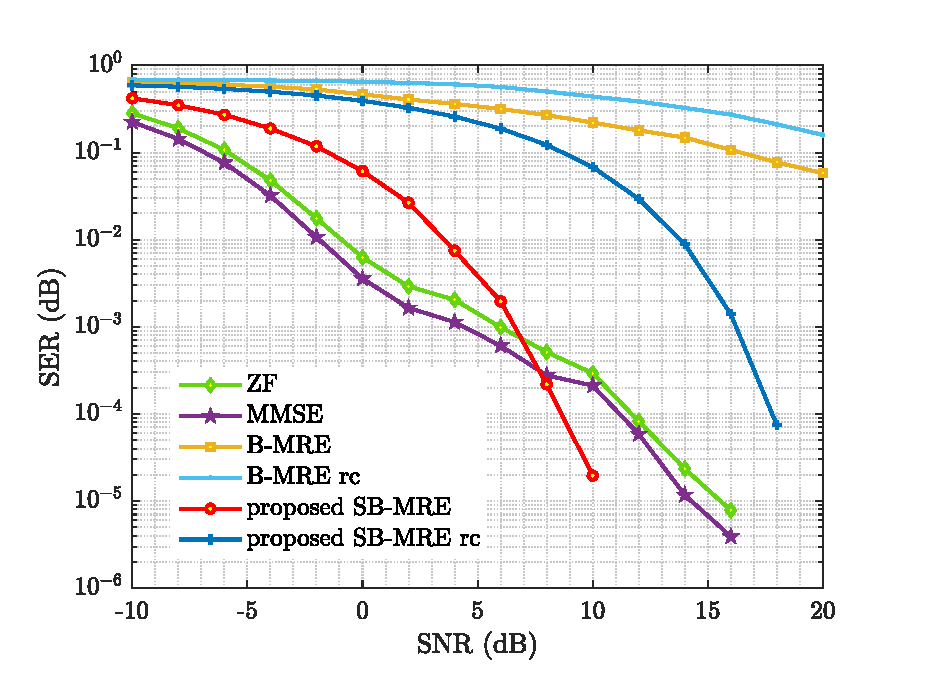
\includegraphics[width=.8\linewidth]{figures/performance.eps}
    \caption{Proposed SB-MRE for channel estimation.}
    \label{fig:performance}
\end{figure}

After that, we simulate to verify the performance of proposed SB-MRE in different numbers of pilots ($N_p$) and SNR values. As shown in Fig.~\ref{fig:vary_N_p}, $N_p$ and SNR are turned in range $[10 \;\; 64]$ pilot symbols and $[5, 10, 15]$~dB, respectively. Overall, the SER curves of SB-MRE and SB-MRE\_rc gradually decrease when $N_p$ and SNR are larger. The behavior is the trade-off between spectrum efficiency and the accuracy of channel estimation algorithm. At $\text{SNR}=15~\text{dB}$, SB-MRE with $N_p > 30$ archives to perfect SER. For SB-MRE\_rc, when $N_p$ increases in range $[10 \;\; 20]$, SER curves clearly improve. But if $N_p > 20$, the SER curves almost keep stable. 
\begin{figure}[ht]
    \centering
    \begin{subfigure}
         \centering
         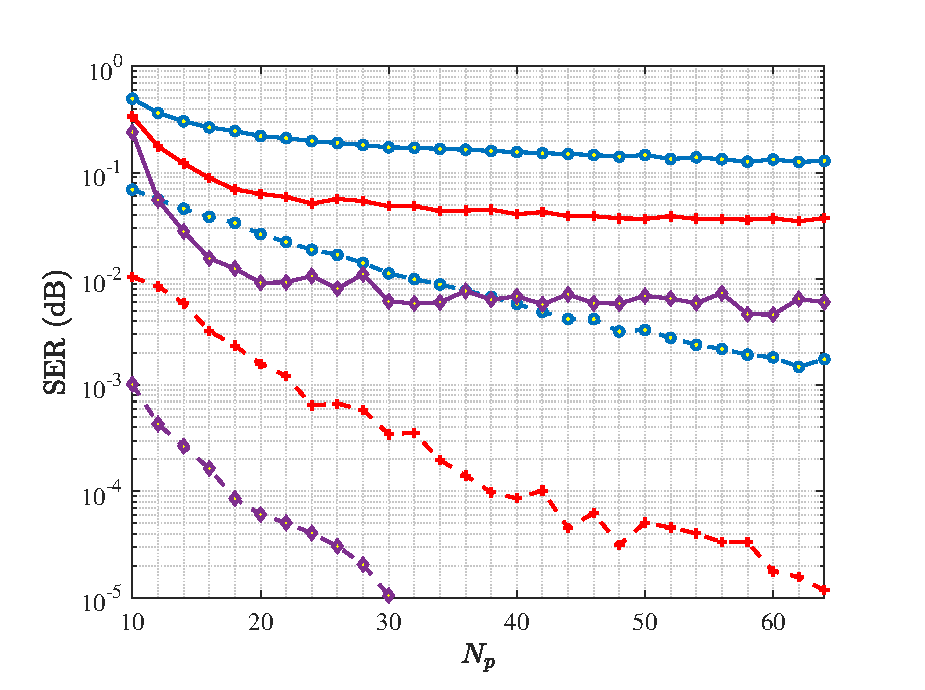
\includegraphics[width=0.8\linewidth]{figures/vary_N_p_1.eps}
     \end{subfigure}
     \hfill
     \begin{subfigure}
         \centering
         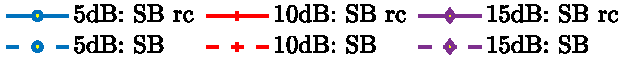
\includegraphics[width=.6\linewidth]{figures/legend.pdf}
     \end{subfigure}
     \hfill
    \caption{Performance of proposed SB-MRE with differs $N_p$ and SNR.}
    \label{fig:vary_N_p}
\end{figure}

Finally, we consider the effect of weighting factor ($\lambda$) between pilot-based and B-MRE. The $\lambda$ is turned in range $[0.01 \;\; 0.2]$. As illustrated in Fig.~\ref{fig:vary_lambda}, at lower SNR, i.e., $5, 10$~dB, the SER curves slightly reduce as $\lambda$ increases. However, $\text{SNR}=15~\text{dB}$, the B-MRE component's performance becomes significant, leading to the SER curve of SB-MRE\_rc markedly decreasing. At the same SNR level, the proposed SB-MRE gets perfect accuracy, as shown in Fig.~\ref{fig:performance}.

\begin{figure}
    \centering
    \begin{subfigure}
         \centering
         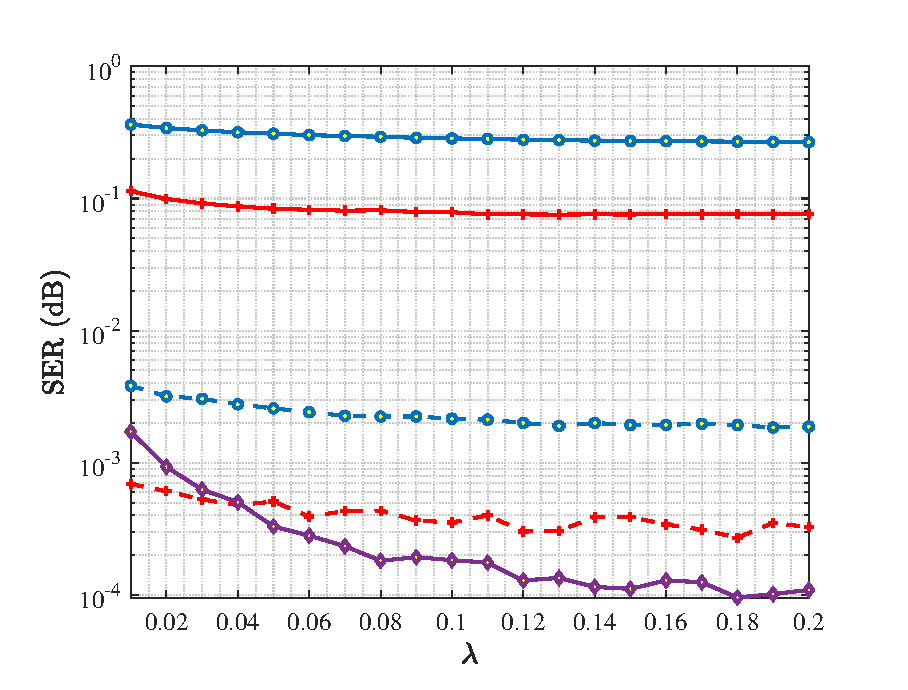
\includegraphics[width=.8\linewidth]{figures/vary_lambda.eps}
     \end{subfigure}
     \hfill
     \begin{subfigure}
         \centering
         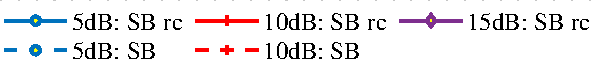
\includegraphics[width=.6\linewidth]{figures/legend_1.pdf}
     \end{subfigure}
     \hfill
    \caption{Performance of proposed SB-MRE with differs $\lambda$ and SNR.}
    \label{fig:vary_lambda}
\end{figure}
	\newpage
	\clearpage
\phantomsection

\setcounter{chapter}{2}
\chapter[NHẬN DẠNG HỆ THỐNG SỬ DỤNG MẠNG HỌC SÂU]{Nhận dạng hệ thống sử dụng mạng học sâu}

	% \newpage
	% \clearpage
\phantomsection

\setcounter{chapter}{3}
\chapter[KẾT QUẢ MÔ PHỎNG]{Kết quả mô phỏng}
	\newpage
	\clearpage
\phantomsection

\addcontentsline{toc}{chapter}{KẾT LUẬN}
\chapter*{Kết luận}
	\newpage
	\clearpage
\phantomsection

\addcontentsline{toc}{chapter}{DANH MỤC CÔNG TRÌNH KHOA HỌC CỦA TÁC GIẢ LIÊN QUAN ĐẾN LUẬN VĂN}
\chapter*{DANH MỤC CÔNG TRÌNH KHOA HỌC CỦA TÁC GIẢ LIÊN QUAN ĐẾN LUẬN VĂN}

\noindent Kết quả nghiên cứu của chương~\ref{sec:CRB} đã được công bố:
\begin{enumerate}
    \item[] \textbf{Do Hai Son} and Tran Thi Thuy Quynh (2023), ``Impact Analysis of Antenna Array Geometry on Performance of Semi-Blind Structured Channel Estimation for massive MIMO-OFDM systems,'' in \textit{IEEE Statistical Signal Processing Workshop (SSP)}, Hanoi, Vietnam, July. [accepted]
\end{enumerate}

% \noindent Kết quả nghiên cứu liên quan khác:
% \begin{enumerate}
%     \item[] \textbf{Do Hai Son} and et al. (2023), ``On the Semi-Blind Mutually Referenced Equalizer for MIMO Systems,''  \textit{Asia-Pacific Signal and Information Processing Association – Annual Summit and Conference (APSIPA-ASC)}, Taipei, Taiwan, November. [submitted]
% \end{enumerate}

	\def\baselinestretch{1}
	
	\vspace{-2cm}
	\clearpage
	\phantomsection
	\addcontentsline{toc}{chapter}{TÀI LIỆU THAM KHẢO}
	\renewcommand{\bibname}{Tài liệu tham khảo}
	
	% Tài liệu tham khảo
	
	\bibliographystyle{./footage/agsm_uet.bst}
	\bibliography{library.bib}
	
	\newpage
	\appendix
	\clearpage
\phantomsection

\addcontentsline{toc}{chapter}{PHỤ LỤC}
\chapter*{Phụ lục}

\renewcommand{\thesection}{\Alph{section}}

\section{Thuật toán tối ưu Adam}
\label{sec:adam}
Thuật toán tối ưu Adam là phương pháp tối ưu hơn so với giải thuật tối ưu giảm dần độ dốc ngẫu nhiên (SGD - Stochastic gradient descent). Adam áp dụng các tốc độ học tập thích nghi ($\delta$ - Adaptive learning rate) khác nhau cho mỗi tham số học. Điều này mang lại lợi thế lớn khi các mô hình mạng nơ-ron với kiến trúc phức tạp. Một số phần trong mạng nơ-ron nhạy cảm với sự thay đổi của trọng số theo các cách riêng biệt. Do vậy, các phần này sẽ cần tốc độ học nhỏ hơn với các vùng khác. Trong luận văn này, tác giả chỉ đưa ra một số biểu diễn toán học quan trọng của Adam, chi tiết về giải thuật tối ưu này có tại~\cite{Diederik2014}.

\begin{subequations}
    \begin{align}
        m_t &=\beta_1 m_{t-1}-\left(1-\beta_1\right) g_t  \tag{$\text{A.a}$}\\
        v_t &=\beta_2 v_{t-1}-\left(1-\beta_2\right) g_t^2 \tag{$\text{A.b}$}\\
        \hat{m}_t &=\frac{m_t}{1+\beta_1^t} \tag{$\text{A.c}$}\\
        \hat{v}_t &=\frac{v_t}{1+\beta_2^t} \tag{$\text{A.d}$}\\
        w_t &= w_{t-1}-\delta \frac{m_t}{\sqrt{\hat{v}_t}+\epsilon} \tag{$\text{A.e}$}
    \end{align}
\end{subequations}
trong đó:
\begin{itemize}[-]
    \item  $\delta$: tốc độ học.
    \item  $\beta_1, \beta_2$: tỉ lệ giảm dần theo cấp số nhân cho ước lượng moment thứ nhất và hai.
    \item  $m_t$: giá trị trung bình của ước lượng moment thứ nhất.
    \item  $v_t$: phương sai của ước lượng moment thứ hai.
    \item  $g_t$: gradient.
    \item  $\hat{m}_t$: các công cụ ước lượng hiệu chỉnh bias cho moment thứ nhất.
    \item $\hat{v}_t$: các công cụ ước lượng hiệu chỉnh bias cho moment thứ hai.
    \item $w_t$: trọng số của mô hình.
\end{itemize}
\end{document}